\section{Analysephase}
\label{sec:Analysephase}
In der Analysephase eines Softwareentwicklungsprojekts werden die Anforderungen an das zu entwickelnde System erhoben. Zur Ermittlung der Anforderungen soll eine Datenanalyse und eine Anforderungsanalyse durchgeführt werden, die Einblicke in die bisherigen Prozesse der Anwesenheitsplanung geben sollen. Für die Informationsbeschaffung wird auf die Analysemethode der Datenanalyse gesetzt. Um die so gewonnenen Daten zu validieren und auch subjektive Verbesserungsvorschläge zu berücksichtigen, werden Interviews mit den Mitarbeitern abgehalten. Die dabei erhobenen Daten werden anschließend aufbereitet und zur Modellierung von Spezifikationen genutzt. Modelle stellen bei der Softwareentwicklung einen großen Nutzen dar, indem sie die Anforderungen in für den Auftraggeber und den Entwickler interpretierbarer Form abbilden. (vgl. \cite[S. 43]{dumke-2003})

Die folgenden Abschnitte beschreiben die Vorgehensweise und Ergebnisse der durchgeführten Analysen. Die dabei gewonnenen Erkenntnisse bilden die Grundlage für die weiteren Entscheidungen für die Umsetzung des Projektes.


\subsection{Analyse des Ist-Zustandes}
\label{sec:Ist-Zustand}
Um eine verbesserte Variante eines Anwesenheitsplaners zu erstellen, ist es notwendig, die bestehenden Systeme und Abläufe zu verstehen. Dafür wurden Interviews mit Mitarbeitern aus verschiedenen Referaten geführt und analog dazu die verschiedenen Excel-Dateien analysiert. Dabei lag der Fokus auf der Analyse des Prozesses der Anwesenheitsplanung, um diesen durch die neue Variante des Anwesenheitsplaners bestmöglich zu unterstützen.

Die Interviews ergaben, dass das Excel-Dokument meist in einem Netzlaufwerk aufbewahrt wird, um für alle Referatsmitglieder zugänglich zu sein. Das Dokument wird nicht anders behandelt als andere Referatsdaten, was bedeutet, dass es keine spezielle Rechteverwaltung gibt. Das kann zu Fehlern und Inkonsistenzen durch versehentliches Ändern von Datensätze führen, da jeder Mitarbeiter des Referats Schreibrechte für das gesamte Dokument besitzt.

Als primäres Problem wurde die Tatsache, dass nur ein Nutzer gleichzeitig auf das Excel-Dokument zugreifen kann, festgestellt. Das führt dazu, dass auf unbestimmte Zeit keine Möglichkeit besteht, den eigenen Status zu ändern. Meistens tritt der Umstand auf, wenn ein Mitarbeiter die Datei im Hintergrund geöffnet hat, ohne diese aktiv zu nutzen.

Für die Datenanalyse wurden von den beteiligten Referaten eine Kopie ihrer Excel Datei zur Verfügung gestellt. Hauptsächlich sollte der Aufbau der Tabelle und die enthaltenen Informationen untersucht werden. Die Analyse ergab, dass alle Anwesenheitsplaner Tabellen ähnlich aufgebaut sind. Unterschiede zeigten sich meist nur in der Bezeichnung der Anwesenheitszustände und der Granularität der Zeitabschnitte. Um eine Referenz für die weitere Entwicklung zu haben, wurde aus den Referats-Tabellen eine Modelltabelle für die Anwesenheitsplanung erstellt, siehe Abbildung \ref{abb:Ausgangstabelle} im Anhang.

Die neue Lösung sollte die Möglichkeit bieten, dass mehrere Nutzer gleichzeitig auf die Anwesenheitsdaten zugreifen und diese aktualisieren können. Das Einführen eines Rechtesystems und die Integration einer Datenbank könnten die Datensicherheit des Anwesenheitsplaners erheblich verbessern.

\newpage

\subsection{Anforderungen an den Anwesenheitsplaner}
\label{sec:Soll-Zustand}
Basierend auf den in der Ist-Analyse gesammelten Erkenntnissen wird deutlich, dass der Anwesenheitsplaner an vielen Stellen verbessert werden muss. Um die zu Anforderungen an das neue System zu visualisieren, wurde eine Use-Case-Analyse durchgeführt. Dabei wird das gewünschte Verhalten der Software dem Nutzer gegenüber als Anwendungsfall spezifiziert. Aus der Summer aller Nutzungsfälle lässt sich dann die gewünschte Funktionalität der Software ableiten, ohne dabei auf konkrete Realisierungsschritte eingehen zu müssen.(vgl. \cite[S. 164]{neumann-2002})

\begin{figure}[htb]
    \centering
    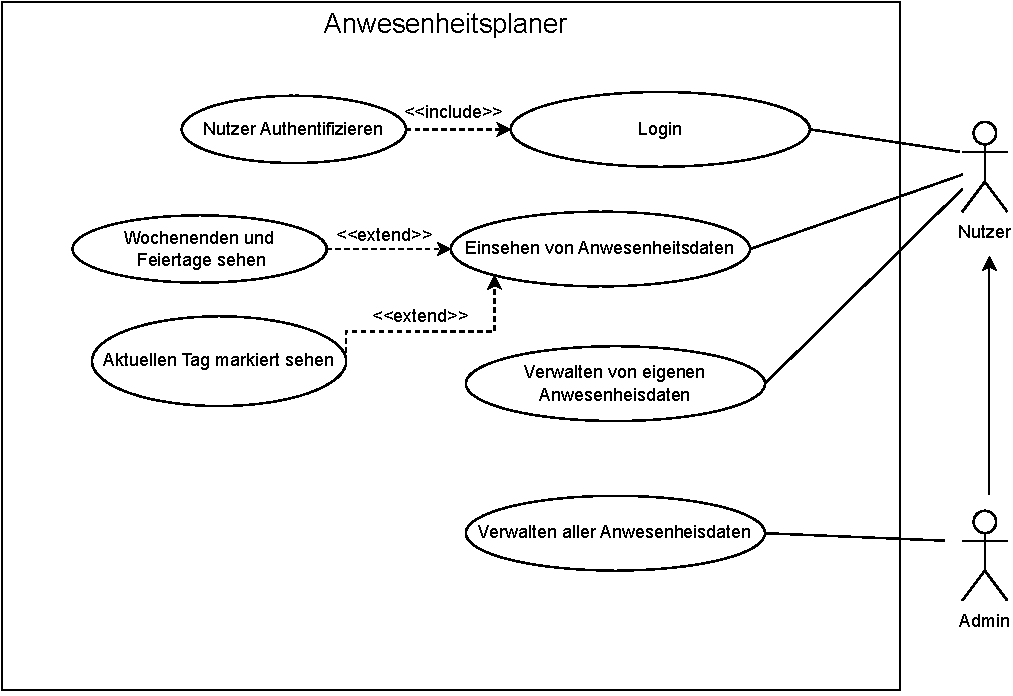
\includegraphics[width=0.7\textwidth,angle=0]{abb/use-case-diagramm.pdf}
    \caption[Use-Case-Diagramm]{Use-Case-Diagramm}
    \label{fig:Use-Case-Diagramm}
\end{figure}

Aus dem Use-Case-Diagramm in Abbildung~\ref{fig:Use-Case-Diagramm} geht hervor, das ein Nutzer sich am System anmelden können, soll um Anwesenheitsdaten seines Referates zu sehen und eigene Daten zu verwalten. Das Verwalten soll das Erstellen, Bearbeiten und Löschen von Einträgen beinhalten. Des Weiteren wird auch ein zweiten Nutzertyp benötigt, der als Admin fungiert und Einträge von anderen Mitarbeitern des Referates ändern kann.

Aus den Interviews konnten noch weitere Spezifikationen ermittelt werden. Am wichtigsten ist die Möglichkeit des Mehrbenutzerzugriffs. Die neue Software sollte es ermöglichen, mehrere Benutzer gleichzeitig auf den Anwesenheitsplaner zugreifen und ihre Daten aktualisieren zu lassen. Dadurch werden Engpässe bei der Aktualisierung der Anwesenheitsdaten vermieden und die Benutzerfreundlichkeit verbessert. Um die Benutzerfreundlichkeit noch weiter zu verboptimieren, soll eine ähnliche Benutzeroberfläche wie die der Excel Tabelle entstehen, die zusätzlich das Eintragen der Datensätze durch \zB Mehlfachauswahl vereinfacht.

\newpage

Zudem sollen Datenschutz und Datensicherheit im neuen System gewährleistet werden, indem Sicherheitsmaßnahmen vor unbefugtem Zugriff oder Verlust der Daten schützen. Es werden Mechanismen zur Datensicherung und Benutzer-Authentifizierung benötigt, um zu gewährleisten, dass Benutzer nur auf die Daten zugreifen und Änderungen vornehmen können, für die sie autorisiert sind.

Um das geforderte System und dessen Komponenten zu skizzieren wurde ein Paketdiagramm, siehe Abbildung \ref{abb:Paketdiagramm} erstellt. Dieses soll für die Entwurfsphase als Referenz genutzt werden.

\begin{figure}[htbp]
    \centering
    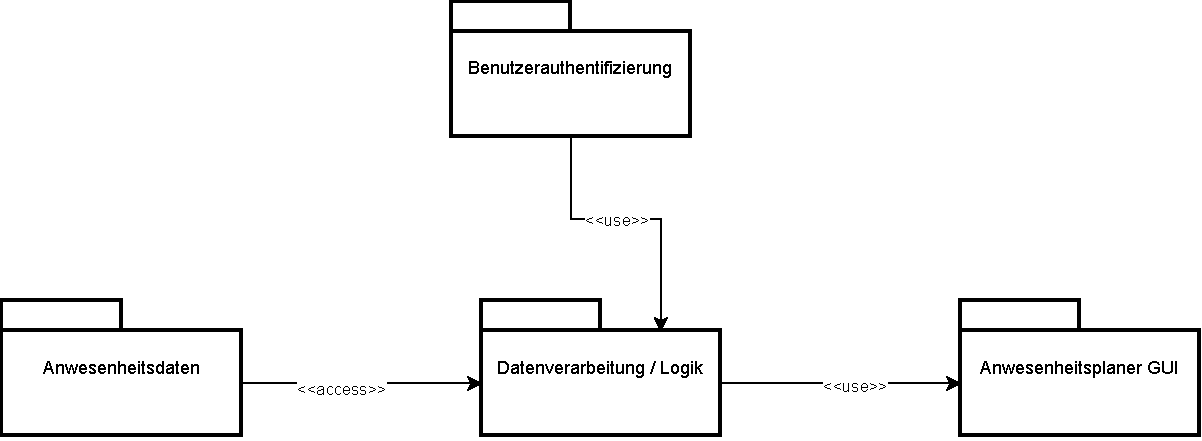
\includegraphics[width=0.7\textwidth,angle=0]{abb/Paketdiagramm.pdf}
    \caption[Paketdiagramm als Skizze das Systems und dessen Komponenten]{Paketdiagramm}
    \label{abb:Paketdiagramm}
\end{figure}

\subsection{Datenschutz und Datensicherheitsbetrachtung}
\label{sec:Datenschutz}
Um das Projekt umsetzten zu können, muss sichergestellt werden, das die Anforderungen an die Informationssicherheit berücksichtigt werden. Dafür wurde in Absprache mit dem Informationssicherheitsbeaufragten des SMK die Orientierung am IT-Grundschutzkompendium des BSI beschlossen.

\subsubsection{Schutzbedarfsfeststellung}
\label{sec:Schutzbedarfsfeststellung}
Um das Maß an zu implementierenden Datensicherheitsmaßnahmen zu ermitteln, wurde eine Schutzbedarfsfeststellung nach BSI-Standard 200-2 durchgeführt. Dabei gilt es, zu ermitteln, welcher Schaden entstehen kann, wenn eines der Grundziele Vertraulichkeit, Integrität oder Verfügbarkeit verletzt wird. Diese drei Grundziele werden einzeln bewertet und ergeben zusammen den Schutzbedarf des Systems. Dafür gibt es die Schutzbedarfskategorien: normal (überschaubarer Schaden), hoch (beträchtlicher Schaden) oder sehr hoch (katastrophaler Schaden), die dann für die Selektion erforderlichen Maßnahmen in den BSI Umsetzungsrichteinen referenziert werden. (vgl. \cite[S.104 - 109]{BSI200-2})

\begin{table}[htbp]
    \centering
    \caption[Schutzbedarfsanalyse]{Schutzbedarfsanalyse}
    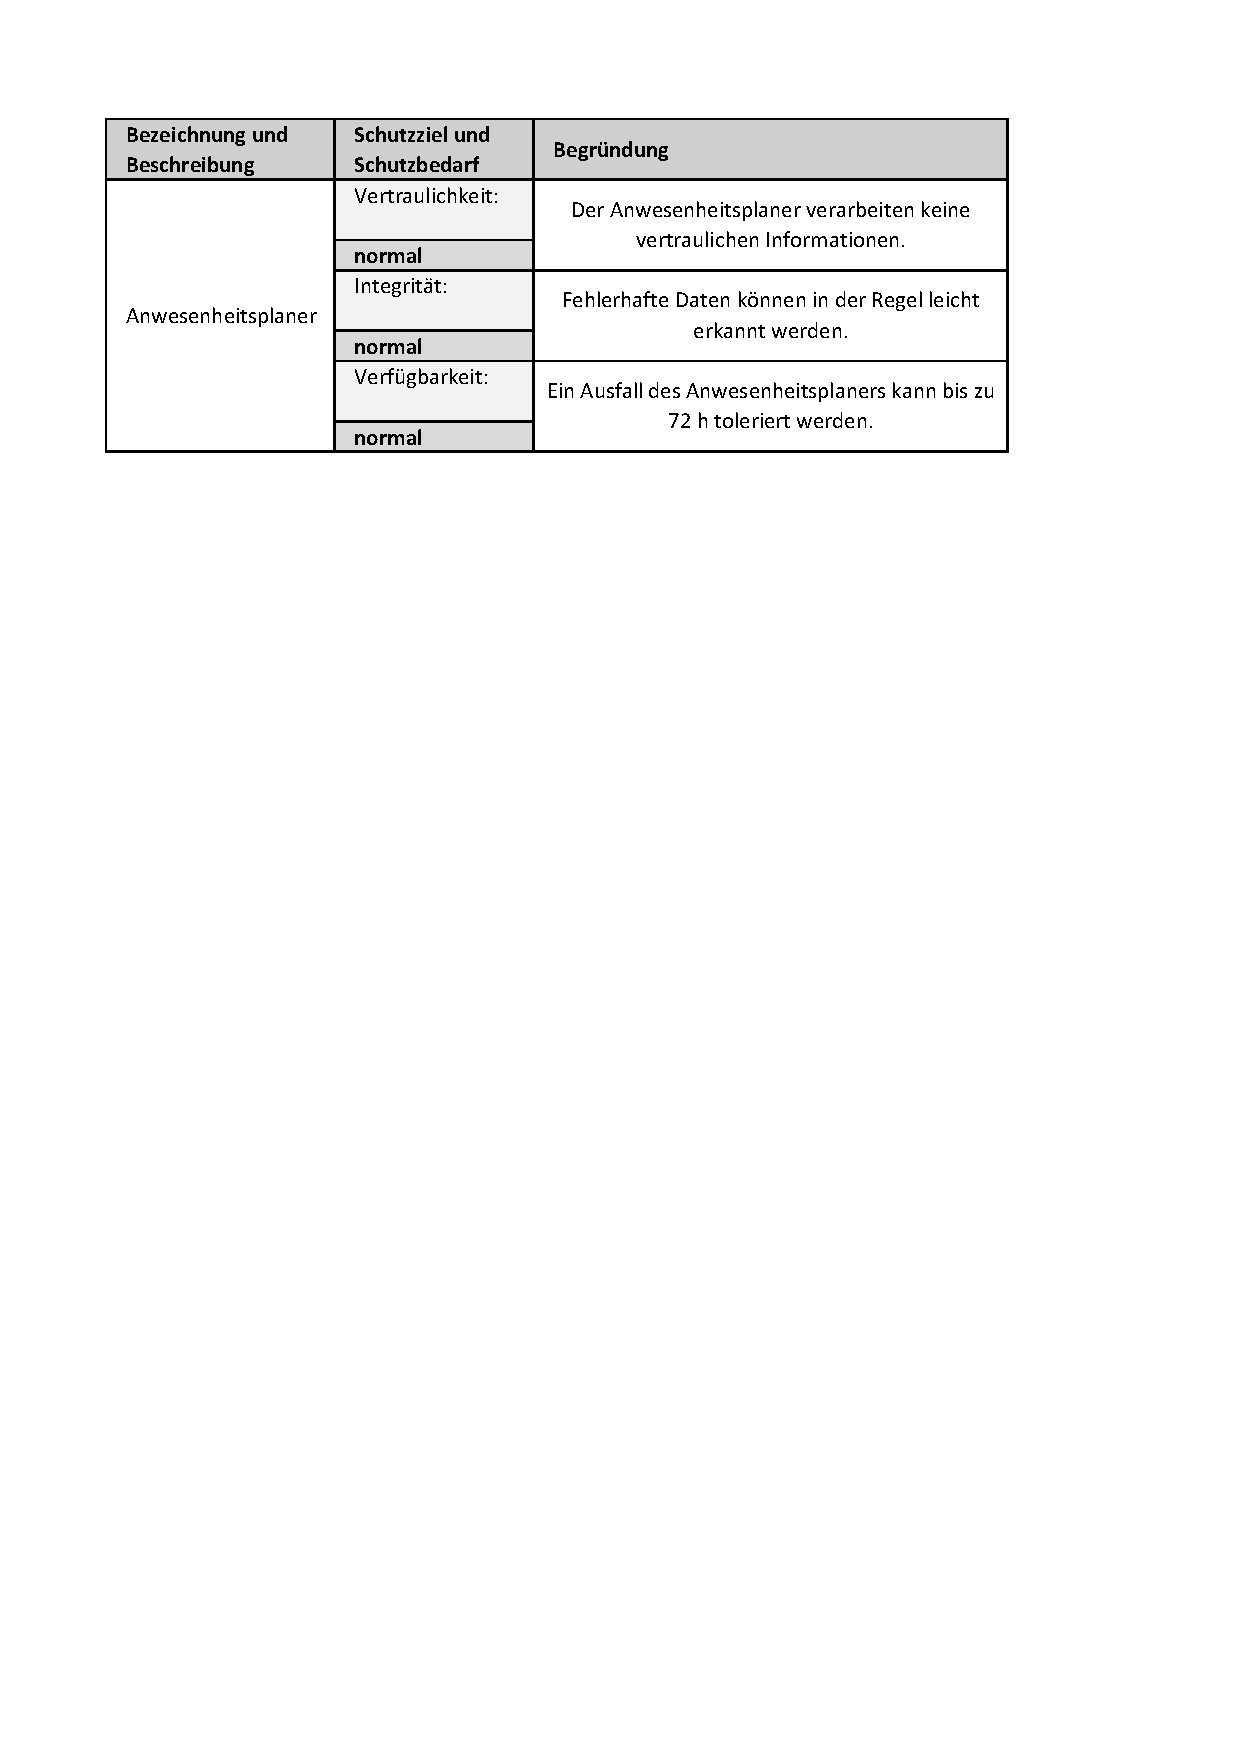
\includegraphics[width=0.7\textwidth,angle=0]{abb/Schutzbedarfsanalyse.pdf}
    \label{abb:Schutzbedarfsanalyse}
\end{table}

Aus der Schutzbedarfsanalyse in Tabelle \ref{abb:Schutzbedarfsanalyse} geht hervor, dass der Anwesenheitsplaner der Schutzbedarfskategorie normal zugeordnet werden kann. Das bedeutet, dass bei der Umsetzung die Basisanforderungen des BSI erfüllt werden müssen. In der Entwurfsphase werden dann die für das entstehende System passende Maßnahmen auf Grundlage der BSI Anforderungen gewählt. Darunter fällt auch der Datenschutz, da die verarbeitete Daten Personen direkt zugeordnet werden können. Dementsprechend müssen auch für die Gewährleistung des Datenschutzes Maßnahmen getroffen werden, welche die Grundanforderungen des Datenschutzes sowie die Umsetzungsrichtlinien der Datenschutzbeauftragten aufgreift. Dabei liegt ein besonderer Fokus auf der Sicherheit der personenbezogenen Daten, sodass diese nur an die dafür autorisierte Benutzer gelangen können.

\subsubsection{Rollen- und Berechtigungskonzept}
\label{sec:RollenBerechtigungskonzept}
Um Benutzern rollenbasierte Rechte zuweisen zu können und eine solche Zugriffskontolle zu gewährleisten, muss ein Rollen- und Berechtigungskonzept erstellt werden. Nach Vorgabe des BSI im Leitfaden zur Entwicklung sicherer Webanwendungen sollte dafür eine Access Control Matrix erstellt werden, die zeigt welche Berechtigungen Rollen auf bestimmte Assets haben. (vgl. \cite[S.26]{BSIWeb})

\begin{table}[htbp]
    \centering
    \caption[Access Control Matrix]{Access Control Matrix}
    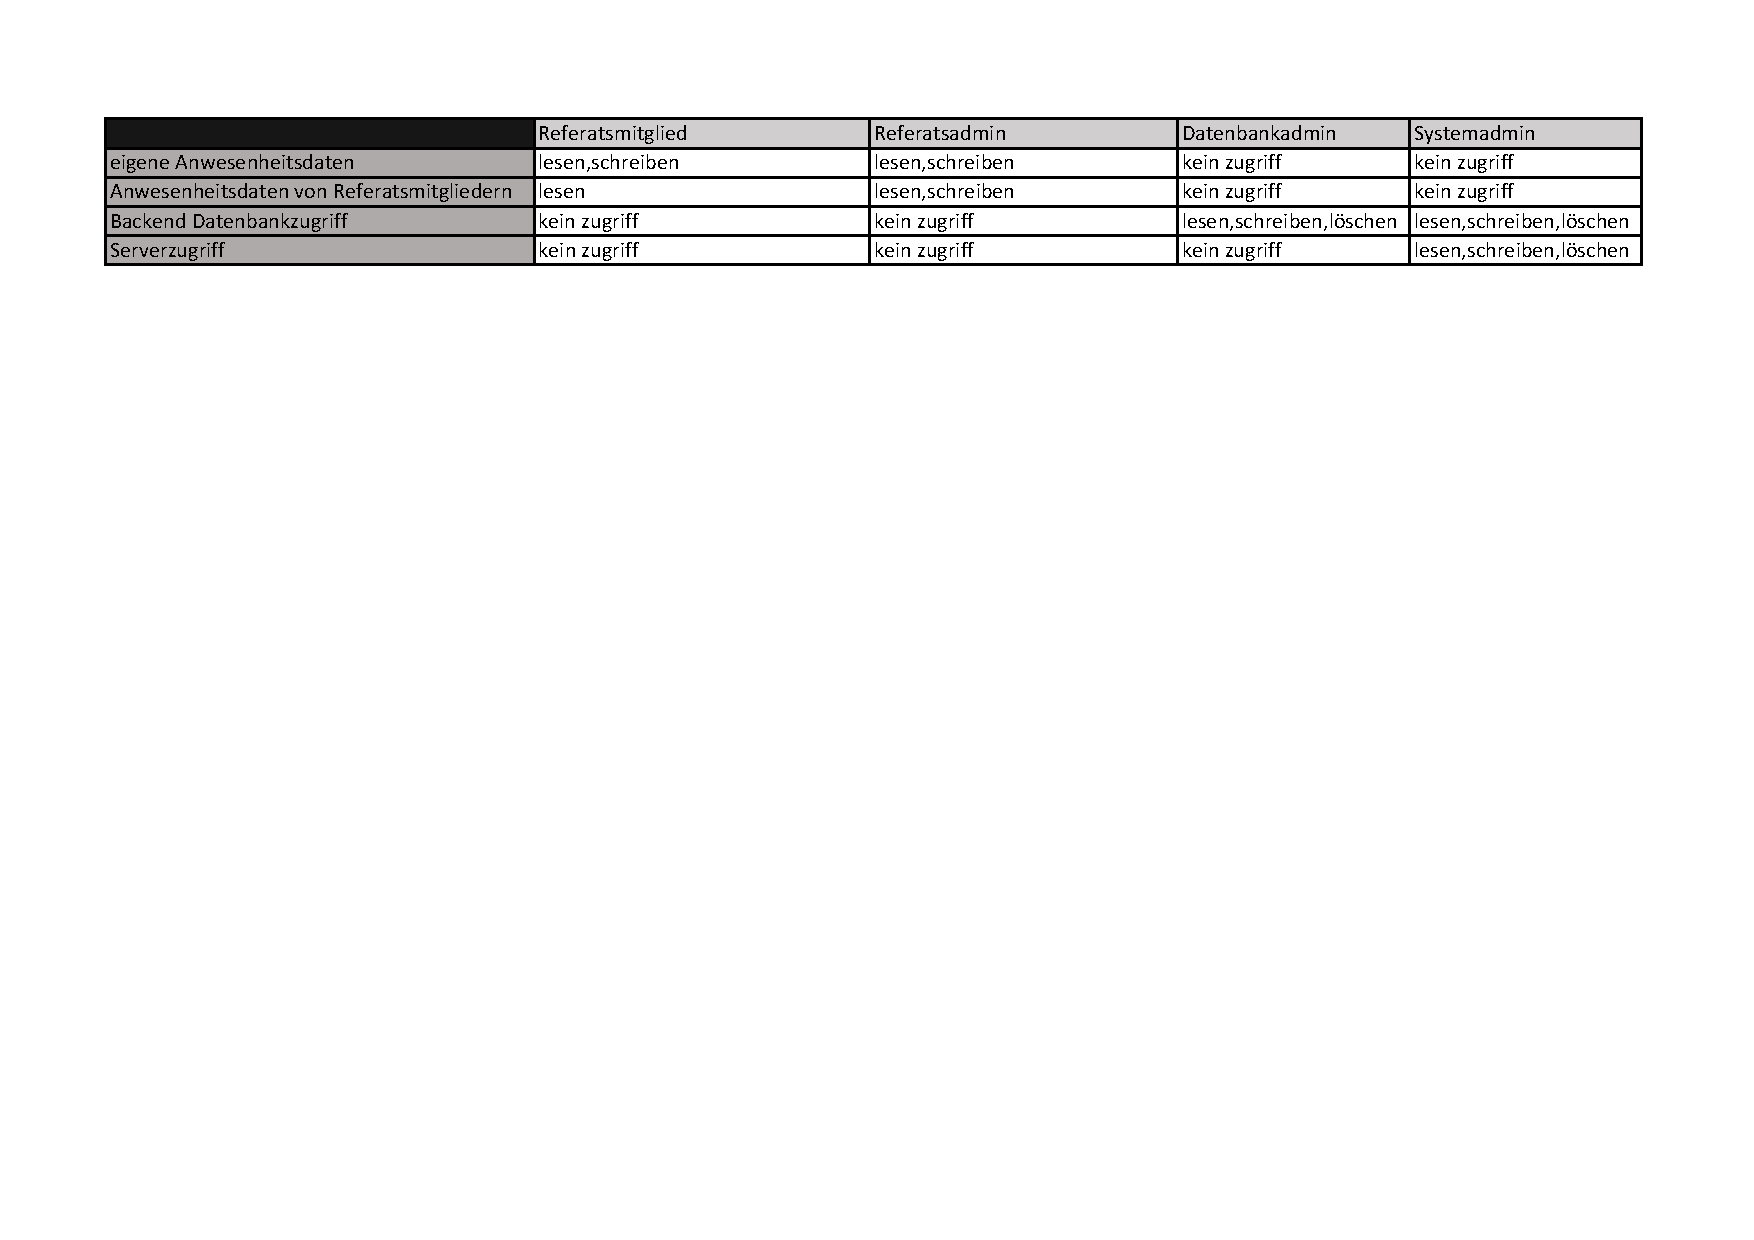
\includegraphics[width=1\textwidth,angle=0]{abb/Berechtigungsmatrix.pdf}
    \label{abb:AccessControlMatrix}
\end{table}

Die erstellte Access Control Matrix setzt sich aus vier Rollen zusammen. Zwei davon sind Nutzerrollen, die anderen zwei Administratorenrollen für die Systeme. Referatsmitglieder sind prinzipiell alle Mitarbeiter des SMK, die einem Referat zugeordnet sind. Diese dürfen eigene Anwesenheitsdaten eintragen und \ggfs ändern. Um für Kollegen die gerade nicht ihre Anwesenheit im System eintragen können, Anwesenheiten zu setzen, gibt es die Rolle des Referatsadmins. Diese Rolle soll über eine Active Directory (AD) Gruppe an die betreffenden Personen ausgerollt werden. Welche Person im Referat diesen Status bekommt, ist den Referaten selbst überlassen.

\newpage

Für die Administration der Systeme sind die Rollen des Datenbank- und des Systemadmins vorgesehen. Dabei lehnt sich das Berechtigungskonzept an die bereits vorhandenen Berechtigungsstrukturen im IT-Referat an. Der Datenbankamin kann im Falle von fehlerhaften Eintragungen oder nötigen Korrekturen, die nicht über den Referatsadmin möglich sind, die Einträge in der Datenbank korrigierten. Für etwaige Wartungs- oder Updatarbeiten am System gibt es den Systemadmin. Er hat Vollzugriff auf alle Systeme und kann Updates oder Wartungsarbeiten ohne Einschränkungen durchführen.